This thesis described efforts in \hl{developing a \emph{software tool for authoring mid-air gestures}} to support the activities of \hl{end-users.} For this purpose, through guidelines derived from the literature and a user-centered design process; \hl{desiderata, design considerations, and evaluation strategies} were uncovered. These led to the development of a user interface paradigm based on space discretization for visualizing and declaratively manipulating mid-air gesture information. This paradigm was \hl{implemented} in Hotspotizer, a standalone Windows application that maps mid-air gestures to commands issued from an emulated keyboard. Hotspotizer was \hl{evaluated} through a user study and class workshop.

\hl{Findings from the evaluation sessions verify that Hotspotizer observes its design rationale and supports gesture authoring for end-users.} Using Hotspotizer, \emph{gestural interactions were implemented by users who did not have the skills} to use textual programming tools. Usage strategies and users' choices for gesture designs implied that users understood the \emph{domain expertise} embedded in the interface and leveraged their \emph{sense of personal space and proprioception} in interacting with the system. Hotspotizer was used to control other programs on a PC, making use of a \emph{common infrastructure}.

Parts of the research described in this thesis have culminated in two academic publications. One is a paper presented at the {Workshop on Engineering Gestures for Multimodal Interfaces (EGMI 2014)}, part of \emph{the sixth ACM SIGCHI Symposium on Engineering Interactive Computing Systems (EICS 2014)} \parencite{Baytas:2014:EGMI}. The other is a forthcoming paper to be presented at and published in the proceedings of \emph{the 8th Nordic Conference on Human-Computer Interaction (NordiCHI '14)} \parencite{Baytas:2014:NordiCHI}.

\section{Revisiting the Research Questions}

The research described in this thesis principally sought to answer \emph{how end-users’ authoring of gross mid-air gestures for skeletal tracking interfaces be supported with a software tool}. One way to enable end-users' authoring of gross mid-air gestures for skeletal tracking interfaces has been found to be with a software tool that implements a user interface paradigm for visually representing and manipulating gesture information by \emph{splitting motion into discrete keyframes} and using \emph{spatial constraints confined to a discrete compartments in a 3-dimensional array.} This method has been observed to be understandable and accessible for end-users designing gestures for current perceptual sensors. Of course, as user interface technologies change over time, the benefits and drawbacks associated with this approach and other methods of authoring gestures may have to be reassessed.

A secondary research question was \emph{specifying the desiderata and design considerations that would pertain to mid-air gesture authoring software for end-users.} The necessary and desirable features for the gesture authoring tool were determined through \emph{formative studies} that comprised workshops with \emph{focus groups} where feedback was gathered using \emph{prototypes} of varying levels of fidelity. The production of the initial prototypes, as well as the formulation of the findings from these studies were directed by \emph{design guidelines derived from previous research}. Nonetheless, while the processes I employed seem to have produced good results; as \textcite{Zimmerman:2007} would concur, different desiderata and design considerations may also have led to a valid solution.

Finally, another secondary research question regarded the \emph{evaluation} of the tool. Whether or not the final artifact observed its design rationale and fulfilled its purpose as an enabler for end-users and a rapid prototyping tool for designers was evaluated through \emph{summative studies} comprising a \emph{user study} with 5 participants and a \emph{classroom workshop} with 6 design students. All participants successfully completed the given tasks, confirming that the design fulfills the aforementioned criteria. Qualitative findings from these studies inform subsequent iterations on the software and highlight opportunities for future work. However, due to issues set forth by \textcite{Olsen:2007} and discussed in Section~\ref{sec:design-and-evaluation-of-tools}, structured usability tests that yield comparable quantitative results have not been conducted with Hotspotizer. This exposes an opportunity for future research on the evaluation of novel intelligent interfaces from a design perspective.

\begin{SCfigure}[\sidecaptionrelwidth][t]
\centering
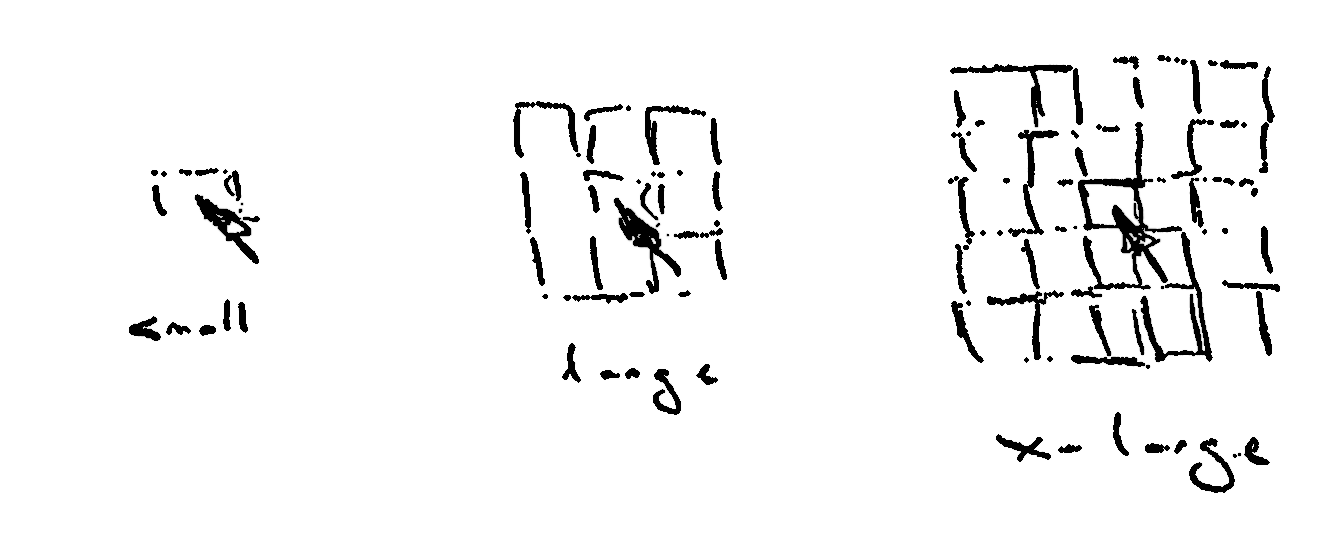
\includegraphics[width=.5\textwidth]{brush}
\caption{An early stage design sketch for a new feature: adjustable brush size may support overcoming users' tendency to spatially overconstrain gesture designs.}
\label{fig:brush}
\end{SCfigure}

\section{Revisiting the Hypothesis and Contributions}

Revisiting my \hl{hypothesis} for the accomplishments of a successfully designed tool for authoring skeletal tracking gestures; evaluations demonstrate that my design accomplishes the following:

\begin{itemize}
\item Hotspotizer \hl{enables \emph{end-users} with no experience in textual programming and/or gestural interfaces to introduce gesture control} to computing applications that serve their own goals. Results from a summative user study with 5 participants and a classroom workshop with 6 participants, described in Section~\ref{sec:summative-studies}, confirm this: Participants without prior experience in developing gesture-based interfaces have successfully completed gesture authoring tasks and demonstrated an understanding of related concepts in usage strategies and post-study interviews. These results are based on qualitative findings. As I stated previously, per \posscite{Olsen:2007} recommendation, Hotspotizer has not been subjected to usability tests that would lead to structured, quantitative, comparable results. This highlights an opportunity for future research on methods the structured evaluation of novel tools.
\item The application \hl{provides \emph{developers} and \emph{designers} of gestural interfaces with a rapid prototyping tool} that can be used to experientially evaluate designs. It has been used precisely for this purpose at a workshop with 6 participants in the context of a design-oriented classroom (Section~\ref{sec:summative-studies}). Design students have implemented prototypes of gesture-based interfaces using Hotspotizer as part of their workflow. As perceptual interactions become pervasive, future research can focus on getting feedback from professional designers and programmers with experience with these technologies.
\end{itemize}

As expected, Hotspotizer fulfills the criteria proposed by \textcite{Zimmerman:2007} for the evaluation of \hl{research-through-design artifacts} \parencite{Frayling:1993}. The design and development \emph{process} employs methods that have been selected rationally and documented in this manuscript. Various topics have been integrated in a novel fashion to create an artifact with the qualities of an \emph{invention.} The resulting artifact, Hotspotizer, demonstrates \emph{relevance}. It is situated within a real, current context; while supporting a shift towards a justifiably preferable state. Finally, the work is \emph{extensible}, as it enables the future exploitation of the knowledge derived from it. Extensible insights gained during design, development and evaluation are documented in this thesis, and the software has been made freely available for use.

The contributions of this work, as expected, are as follows:

\begin{enumerate}
\item The \emph{primary contribution} from this work is, \emph{Hotspotizer}, a \emph{software application} that encompasses an end-to-end solution to authoring mid-air gestures for skeletal tracking input devices. The application accomplishes its previously stated goals of enabling end-users and supporting the activities of designers, and constitutes an authentic contribution as an artifact of research through design. The latest stable release of Hotspotizer's can be obtained online as a free download, for use under the MIT license.
\item \emph{Insights that may inform future interaction design research and practice} have been derived from the design, development, deployment and evaluation of the gesture authoring software. Principally, it has been found that the discretization of both spatial and temporal aspects of gestures contributes to an appropriate user interface paradigm for representing and manipulating gesture information.
\end{enumerate}

\begin{SCfigure}[\sidecaptionrelwidth][t]
\centering
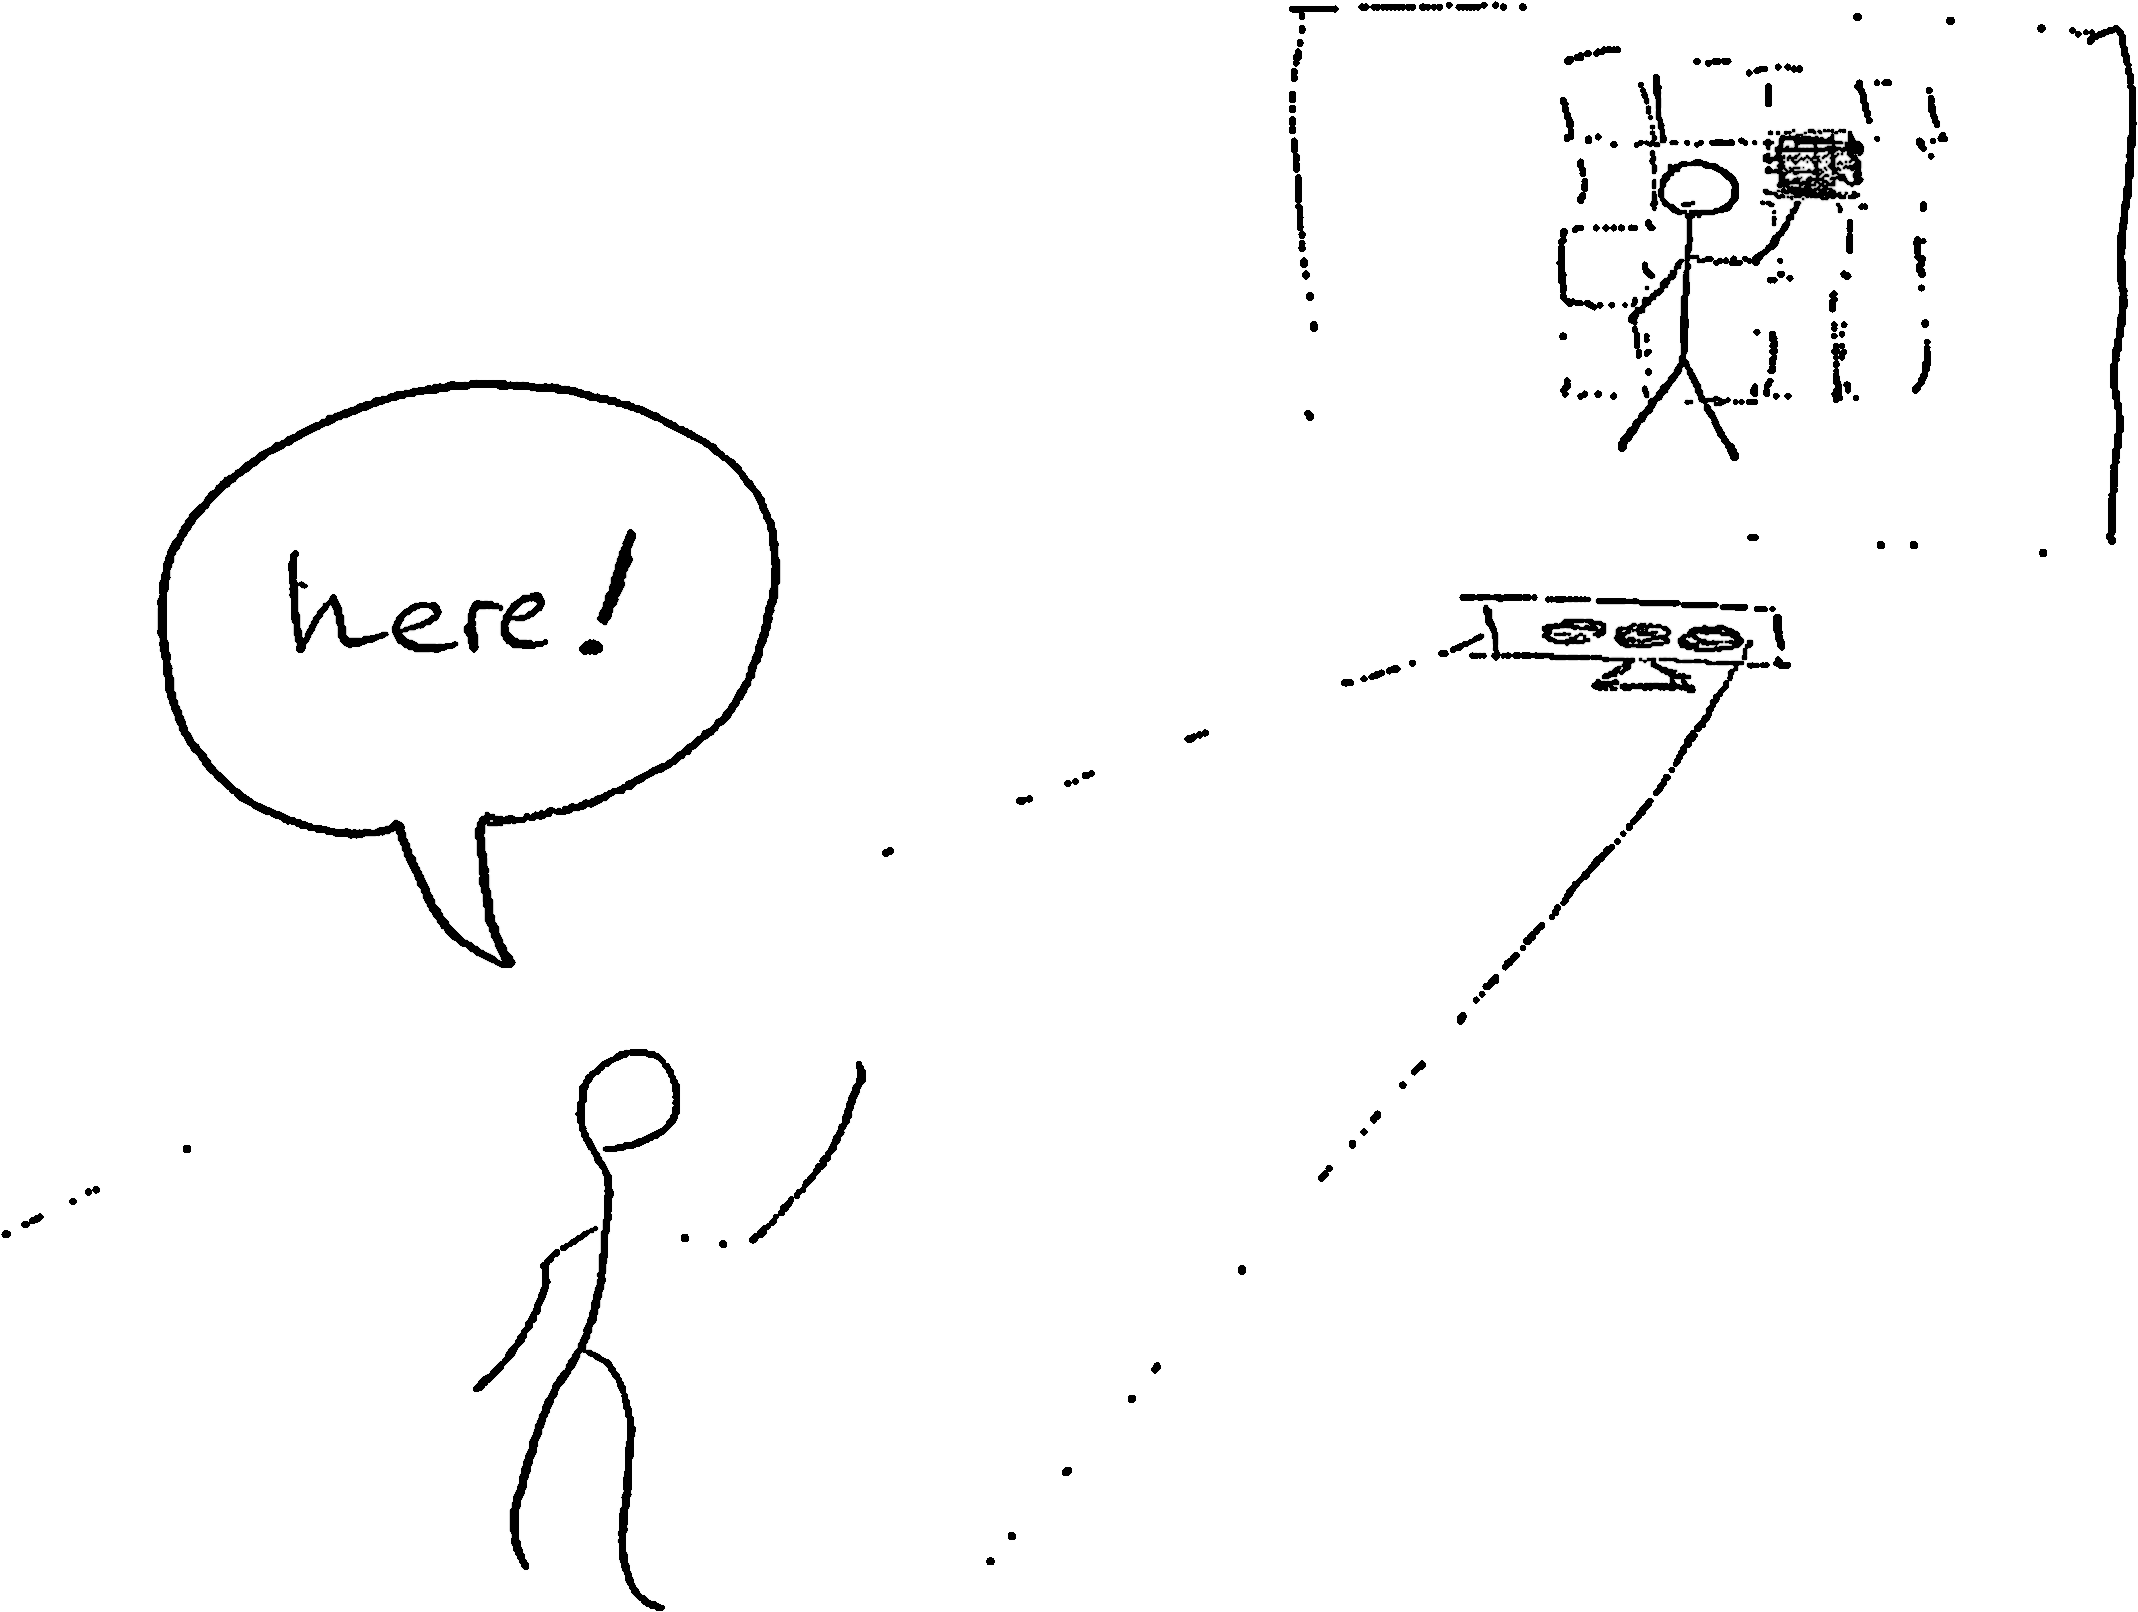
\includegraphics[width=.5\textwidth]{speech-recognition}
\caption{An early stage design sketch for a new feature: inferring hotspots from demonstration while controlling segmentation via a speech interface.}
\label{fig:speech-recognition}
\end{SCfigure}

\section{Future Work}
\label{sec:future-work}

The research described in this thesis instigates a number of opportunities for future work. These opportunities can be examined in two broad categories. First, Hotspotizer can be expanded and improved by addressing a number of technical and design challenges that have surfaced during the research described in this thesis. Second, the space discretization paradigm for authoring gestures can be evaluated, refined and adapted for use with a wider variety of input devices.

\subsection{Expanding Hotspotizer}

One strand of future work may deal with expanding the expressive power of Hotspotizer by implementing new features in a user-friendly manner.

While it did not come up in the user studies, I find that the current visualization style may become convoluted as gesture collections grow in size. Exploring alternative ways of visualizing many gestures within one workspace is on our agenda for future versions of the software.

Currently, (as I discussed in Section~\ref{sec:hotspotizer}) Hotspotizer does not directly support "online" (REF) --- i.e. continuous --- gesturing, since it adopts a traditional event-based model for detecting and responding to gestures. As such, support for \emph{manipulative} and \emph{deictic} gestures, which are common across gesture-based user interfaces, is severely limited. As \textcite{Myers:2000} recommend, ideally, the "continuous nature of the input [should] be preserved." This, however, requires "tighter integration with application logic" \parencite{Hartmann:2007} through interfacing with a textual programming language or third-party applications integrating support for continuous input streams. Unfortunately,  the first option oversteps the scope of the Hotspotizer project (See Section~\ref{sec:scope}). The second option can be explored for a limited set of third-party applications.

Among other features are negative hotspots that mark space that should not be engaged when gesturing (i.e. negation \parencite{Hoste:2014}), a movable frame of reference for the workspace to enable gesturing around peripheral body parts, resizable hotspot boundaries, adjustable timeout, compositions that involve multiple limbs, and recognition of hand movements.  As implied by user studies, the capability to infer hotspots from \emph{demonstration}, and \emph{speech recognition} to control the application from a distance are features that may further accelerate user workflows (Figure\ref{fig:speech-recognition}).

Incorporating classifier-coupled gesture recognition \parencite{Hoste:2013} could serve to alleviate recognizer errors \parencite{Myers:2000}, and, when needed, to decouple overlapping gesture definitions.

Studies have revealed a tendency among users to initially overconstrain gesture designs in terms of spatial restrictions; i.e. users tend to begin with gesture designs that utilize too few hotspots (see Section~\ref{sec:summative-studies}). To steer away users from this tendency, the size of the cursor --- or "brush" --- for marking hotspots could be made adjustable; with the default size being set to mark a larger area and the finer brush made accessible as an option (Figure~\ref{fig:brush}).

\subsection{Space Discretization}

A second strand of future work may focus on evaluating and refining the space discretization paradigm.

The usability and expressive power of the user interface paradigm is independent from its implementation. However, due to various factors that constrain its scope, this work does not evaluate the paradigm separately. In order to refine the user interface paradigm and support implementations in different contexts, user studies can be conducted to evaluate the difficulty of understanding and manipulating gestures visualized as hotspots in discretized space. \textcite{Kin:2012} have conducted a study that examines the speed and accuracy of users' understanding various representations for touch gestures. A similar study that examines representations of gross gestures may inform future work on gesture authoring and documentation.

The space discretization paradigm may also have value for authoring gestures enabled using technologies other than skeletal tracking. I encourage designers, developers, and researchers to adopt the paradigm for use in different contexts.
